\documentclass[a4paper,11pt]{article}
\usepackage[T1]{fontenc}
\usepackage[english]{babel}
\usepackage[utf8]{inputenc}
\usepackage{graphicx}
\usepackage{caption}
\usepackage{subfigure}
\usepackage{indentfirst}
\usepackage{url}
\graphicspath{{Figures/}}
\usepackage{setspace}
\usepackage[a4paper,left=1cm,right=1cm,top=2cm,bottom=2cm]{geometry}
\usepackage{filecontents}
\usepackage{amsmath}
\numberwithin{equation}{section}
\DeclareMathOperator*{\argmax}{arg\,max}

\author{Kevin WIRTZ}
\title{Benchmarking of machine learning classifiers.}
\begin{document}

\maketitle

\tableofcontents
\newpage

\section{Introduction}
\doublespacing

In the last few years Machine learning gained a lot of interest and this is due to two main reasons. Firstly the new technology which allow us to perfom a lot of operations. The fastest supercomputer has a speed of 93 PFLOPS which means $93*10^{15}$ operation in 1 second. Moreover this processing power is also available to interested scholar thanks to  the fact that we can use GPU to perform operations(for example CUDA). But this processing power means nothing if we don't have any reasons to use it. That's where the second reason comes in play. If we take the example of google, they processed 24 petabytes of data per day in 2014 \cite{google}. In his book Nate Silver (2013) \cite{signalnoise} talks about how IBM estimated, in 2012, that we produced 2.5 quintillion bytes of data per day and at this time 90\% of the data was created during 2010-2012. Because of this, Machine learning started to be used in a lot of domains like biology, facial recognition, self driving cars, and others, with results improving the state of the art. The main goal of machine learning being pattern recognition we can already see the link with Econometrics. In fact the border between both of them is thin and it's really hard to distinguish them. Some authors like Charpentier (2015) \cite{charpentier:hal-01568851} did some work on the subject. Since these methods became popular recently, Applications in economics are still scarce. The goal of this paper is to present, compare and propose a benchmarking of different machine learning algorithm, using statistical test, on a bank rating problematic and compare it to classical econometric results to see the advantages and limits of both methodologies. 

Therefore this paper starts by describing different algorithm, their intuition as well as the mathematics behind them. In the first section we will study support vector machines. The second section will be about random tree forest, and lastly we will discuss artificial neural network. The last section is going to be a comparaison of the different algorithms using statistical tests.


\newpage

\section{Support Vector Machine}\label{sec:first}

\doublespacing

Support Vector Machine (SVM) is a type of algorithm used in machine learning mainly as a classifier. The basic procedure was created by Vapnik in 1963 but was then improved in 1992 \cite{Boser:1992:TAO:130385.130401} and then in 1995 \cite{Cortes:1995:SN:218919.218929}. After these two papers, SVM became popular because it gave better accuracy than neural network in classification tasks (until deep neural network which we will discuss later). The main goal of this section is to go more into the details of the method. To understand SVM we will first discuss the case where we have a linearly separable dataset which will allow for an easier understanding of the logic and also introduce the mathematical notations. Once this is done it will be much easier to generalize and understand what has been done in 1992 and 1995. 


\subsection{Linearly and exactly separable}

We begin this section of support vector machines by a two-class classification problem.

\begin{figure}[htb]%
    \begin{center}
    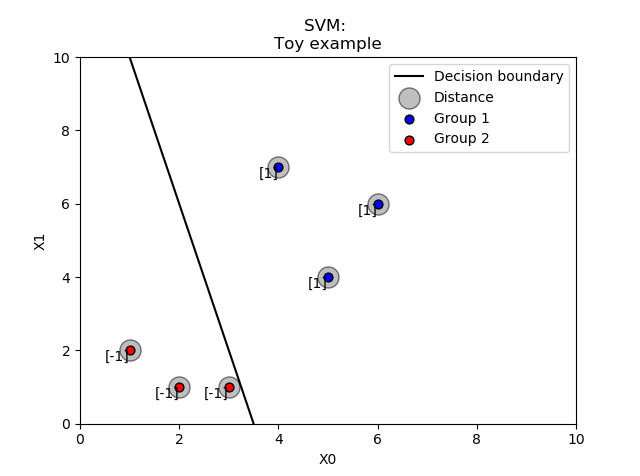
\includegraphics[scale = 0.5]{Figure1SVM.png}%
    \qquad
    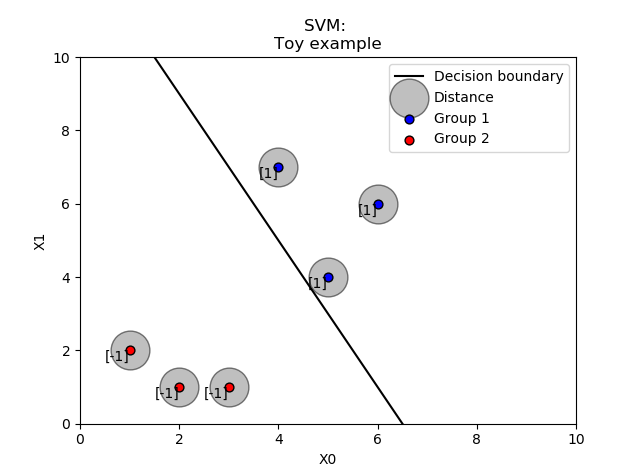
\includegraphics[scale = 0.5]{Figure2SVM.png}%
    \qquad
    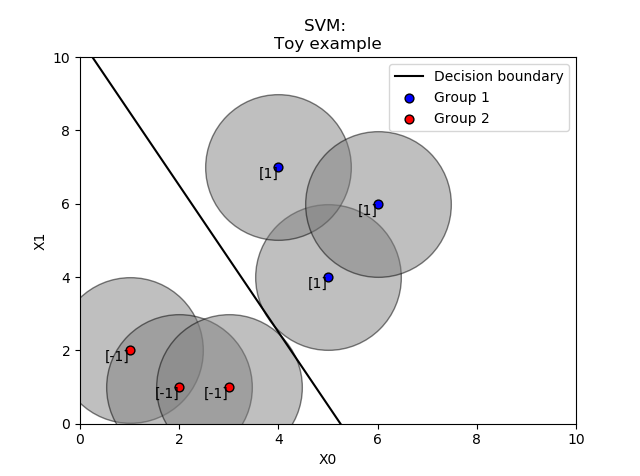
\includegraphics[scale = 0.5]{Figure3SVM.png}%
    \caption{\textbf{Short example of SVM}. \textit{Made with python}}%
    \label{fig:example}%
    \end{center}
\end{figure}

Figure 1 represents a bulk of point with two dimension ($x_1$ and $x_2$) and for two distinct populations (red and blue). The first objective is to code an algorithm which identifies these two groups and separate them by a straight line. To make it easier we will label the group 1 as +1($x_+$ positive example) and group 2 as -1($x_-$ negative example). All figures shows random separating lines, if an observation is over that line it is classified as group 1 and under that line it falls in group 2. But, as a matter of fact, there is an infinite number of separating lines which respect the condition that every observation is correctly classified. Looking at Figure 1, the last one and the reason is that when we get a new observation there's going to be noise and so the new point will be not exactly as the data we used to train. For example if we choose the first line, there's a lot of chance that,if a new negative observation varies just slighty compared to the training set, it will most likely be missclassified to a 1. Therefore we can say that the first line is overfitting.  

\begin{figure}[htb]%
    \begin{center}
    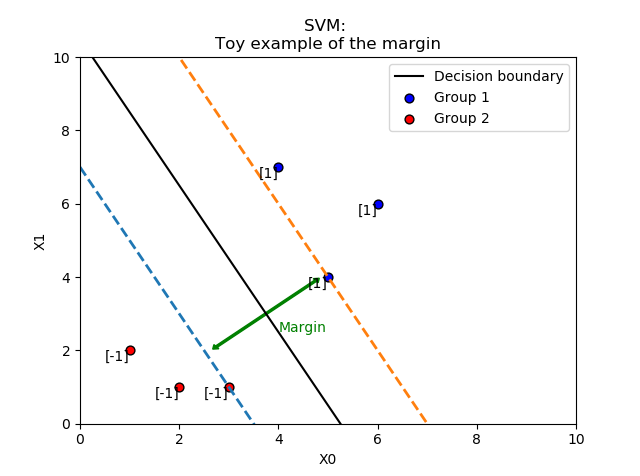
\includegraphics[scale = 0.5]{Figure4SVM.png}%
    \label{fig2:example}%
    \end{center}
\end{figure}

And that's where the SVM procedure introduce the concept of margin/gutter (figure 2). We define the margin as being the minimum distance between this line, also called hyperplan or decision boundary, and any of the observations. What are we going to do with this margin ? We find the maximum margin. So we want to maximize a minimum and by doing that only some points are considered, those who are really close to the hyperplan. Is it something we really want ? To ignore a lots of points ? Indeed it is. The points far away of the decision boundary are not as likely to be falsely classified as the points which are close (look again at the gray area the furthest point could have a bigger circle). So that's the intuition: You have two class, you want to separate them by a line, SVM gives you a line that satisfy a distance criteria.

To do that mathematically we can start by defining an equation for the hyperplan and the decision rule as we do in linear discriminant analysis. Consider $\boldsymbol{\omega}$ as a perpendicular vector,of any length, to the hyperplane and $\boldsymbol{u}$ an unknown which we want to classify. To know the class we just have to project  $\boldsymbol{u}$ on $\boldsymbol{\omega}$. 


\begin{equation*}
\boldsymbol{\omega}\bullet{\boldsymbol{u}} \geq c \mbox{ Then } \boldsymbol{u} \mbox{ is a positive example}
\end{equation*}

Where c is some constant. Note that the $\bullet$ operator, also called dot product, is just the multiplication of two vectors of equal length which returns a scalar. Which means $\boldsymbol{\omega}\bullet{\boldsymbol{u}} = \boldsymbol{\omega}^T{\boldsymbol{u}}$. We can rewrite the first equation this way:

\begin{equation}\label{eq:1}
\boldsymbol{\omega}\bullet{\boldsymbol{u}} + b \geq 0 \mbox{ Then } \boldsymbol{u} \mbox{ is a positive example}
\end{equation}

With $b = -c$. This is called the decision rule where there's 2 unknown $\boldsymbol{\omega}$ and $b$. The only thing we know is that $\boldsymbol{\omega}$ is perpendicular to this hyperplane but there's a lot of perpendicular vector and we still can't choose a particular $\boldsymbol{\omega}$ or $b$. Like we said earlier there might be a lot of line which separates exactly our dataset. The idea would be to find the solution which overfits the less. Now we have to integrate the concept of margin.

\begin{equation}\label{eq:2}
\boldsymbol{\omega}\bullet{\boldsymbol{x_i}} + b \geq 1 \mbox{ if } x_i \mbox{ is in groupe 1}
\end{equation}

\begin{equation}\label{eq:3}
\boldsymbol{\omega}\bullet{\boldsymbol{x_i}} + b \leq -1\mbox{ if } x_i \mbox{ is in groupe 2}
\end{equation}

We will see a bit later that 1 is just a choice born from mathematical convenience. We can introduce an other variable to reduce the systeme of 2 equations in 1

\begin{equation}\label{eq:4}
    y_i = \begin{cases}
               1               & \mbox{if }\boldsymbol{x_i} \in \mbox{group 1}\\
               -1               & \mbox{if }\boldsymbol{x_i} \in \mbox{group 2} \\
           \end{cases}
\end{equation}

Therefore by taking \ref{eq:2},\ref{eq:3} and \ref{eq:4} we obtain

\begin{equation*}
y_i(\boldsymbol{\omega}\bullet\boldsymbol{x_i}+b)\geq 1
\end{equation*}

\begin{equation}\label{eq:5}
y_i(\boldsymbol{\omega}\bullet\boldsymbol{x_i}+b)-1\geq 0
\end{equation}



Now, as a reminder what we are interested in is to maximise the distance between the decision boundary and the closest points. But what is the distance between the hyperplan and an observation? Let's start by taking the vector $\boldsymbol{x}$ unknown and	$\boldsymbol{x}'$ a point in the hyperplan. taking the distance between them and multiplying it by a normalized vector gives us the distance between the hyperplan and the point . We said earlier that $\boldsymbol{\omega}$ is a perpendicular vector, we just need to rescale it to have a unit vector. therefore the distance is just:

\begin{equation}\label{eq:6}
Distance = \frac{\boldsymbol{\omega}}{\|\boldsymbol{\omega}\|}\bullet{(\boldsymbol{x}-\boldsymbol{x}')}
\end{equation}

Mixing the hyperplan equation, which state that if $x'$ is a point on the hyperplan then $\boldsymbol{\omega}^Tx' = -b $, and \ref{eq:6} we find

\begin{equation}\label{eq:7}
Distance = \frac{1}{\|\boldsymbol{\omega}\|}{(\boldsymbol{\omega^T}\boldsymbol{x}+b)}
\end{equation}

Now what we want to keep is the minimum of this distance for both category. We define the width of the gutter as

\begin{equation*}
width = \frac{1}{\|\boldsymbol{\omega}\|}\bullet {\min(y_i(\boldsymbol{\omega}^T\boldsymbol{x_+}+b))}+\frac{1}{\|\boldsymbol{\omega}\|}\bullet {\min(y_i(\boldsymbol{\omega^T}\boldsymbol{x_-}+b))}
\end{equation*}

We just need to find $\omega$ and $b$ which maximise this width. But we can see that the solution would be indifferent to rescaling because of the normalization. Therefore we have the freedom to set the scale and we will choose 1 to facilitate the rest. This explains \ref{eq:5} where we added the constraints. We then rewrite:

\begin{equation}
width = \frac{2}{\|\boldsymbol{\omega}\|}
\end{equation}

Then again we want to maximise this distance but to simplify the program we can change the objective function to

\begin{equation}\label{eq:8}
 \argmax \frac{2}{\|\boldsymbol{\omega}\|} = \argmax \frac{1}{\|\boldsymbol{\omega}\|} = \argmin \|\boldsymbol{\omega}\| = \argmin \frac{1}{2}*\|\boldsymbol{\omega}\|^2
\end{equation}


So now we have the object we want to optimize, our constraint, the next logical step is to carry out a Lagrange optimization

\begin{equation}\label{eq:9}
 \min_{\boldsymbol{\omega},b,\boldsymbol{\alpha}} L= \frac{1}{2}*\|\boldsymbol{\omega}\|^2 - \sum_{i}^{N}\alpha_i[y_i(\boldsymbol{\omega}\bullet{\boldsymbol{x_i}}+b)-1]
\end{equation}

With N being the total of points (we constraint every point to be higher/lower than 1/-1). Solving this yields the next equations:

\begin{equation}\label{eq:10}
 \frac{\partial L}{\partial\boldsymbol{\omega} } = 0 \Longrightarrow \boldsymbol{\omega} - \sum_{i}^{N}\alpha_iy_i\boldsymbol{x_i} = 0 \Longrightarrow \boldsymbol{\omega} =  \sum_{i}^{N}\alpha_iy_i\boldsymbol{x_i}
\end{equation}

\begin{equation}\label{eq:11}
\frac{\partial L}{\partial b}  = 0 \Longrightarrow - \sum_{i}^{N}\alpha_iy_i = 0 \Longrightarrow \sum_{i}^{N}\alpha_iy_i = 0
\end{equation}

Putting \ref{eq:10} and \ref{eq:11} into \ref{eq:9} and simplify gives us the next equation.

\begin{equation}\label{eq:12}
 L = \sum_{i=1}^{N}\alpha_i-\frac{1}{2}\sum_{i}^{N}\sum_{j}^{N}\alpha_i\alpha_jy_iy_j\boldsymbol{x}_i\bullet\boldsymbol{x}_j
\end{equation}

Note that since our counstraint is an inequality this Langrange optimization is actually a Kuhn-tucker optimization and we need to respect the following condition.


\begin{align*}
  \alpha_i \geq 0 \\
  y_i(\boldsymbol{\omega}\bullet{\boldsymbol{x_i}}+b)-1 \geq 0 \\
  \alpha_i[y_i(\boldsymbol{\omega}\bullet{\boldsymbol{x_i}}+b)-1] = 0
\end{align*}

This allow us to discuss the intuition we had at first that not all points will matter, in fact if the points are  not on the margins which means $y_i(\boldsymbol{\omega}\bullet{\boldsymbol{x_i}}+b) > 1 $ then $\alpha_i = 0$ and it won't appear in the sum of the Lagrangian optimization. Only points for which the constraint is equal and are on the margin will have $\alpha_i \geq 0 $ and will have an impact in the solution.

And this is all we need to perform SVM. Something to be aware of is that $L$ is a function of the dot product of pair of observations. Why is it important? The fact is that we started all this discussion by having 2 strong assumptions. One of them is that our datasets is linearly separable. As a matter a fact it's not the case for most of the real world data. That's where the 1992 paper\cite{Boser:1992:TAO:130385.130401} comes in play. 

\subsection{Non linearly and exactly separable}

They released the linear assumption and created a non-linear classifier by using something called the kernel trick. First you have to understand that when we have a non linearly seperable dataset we can transform the different input $x$ and map them in a higher dimensions, we can denote this transformation $\phi(x)$. The only thing that changes when you compare it to the basic procedure is that instead having $\boldsymbol{x}_i$ you have a transformation $\phi(\boldsymbol{x}_i)$. Therefore the dot product in the optimization is transformed into $\phi(\boldsymbol{x}_i)\bullet{\phi(\boldsymbol{x}_j)}$. But this might become computationally too slow. For example

\begin{equation*}
 \boldsymbol{x_i} =
 \begin{bmatrix}
 x_{i1} & x_{i2} 
 \end{bmatrix}^T
\end{equation*}

\begin{equation*}
 \phi(\boldsymbol{x}_i)=
 \begin{bmatrix}
    x_{i1}x_{i1}    & x_{i1}x_{i2} & x_{i2}x_{i1} & x_{i2}x_{i2}\\

 \end{bmatrix}^T \\
 \phi(\boldsymbol{x}_j)=
 \begin{bmatrix}
    x_{j1}x_{j1}    & x_{j1}x_{j2} & x_{j2}x_{j1} & x_{j2}x_{j2}\\

 \end{bmatrix}^T
\end{equation*}

\begin{equation*}
\phi(\boldsymbol{x}_i)\bullet\phi(\boldsymbol{x}_j) = (x_{i1}*x_{i1})*(x_{j1}*x_{j1}) + \dots + (x_{i2}*x_{i2})*(x_{j2}*x_{j2})
\end{equation*}

If we start with a vector of length 2 the transformation give us a vector of length 4 then by doing a dot product we will end up with a scalar. So it's really inefficient. We go in higher dimension (from 2 to 4) and then back to 1. Also it's not unusual to go in even higher dimension. It would be better to go directly from a length 2 to 1. And that's what the kernel trick does. We don't need to know the transformation of a vector we only need to know the dot product of such transformation. let's denote the kernel transformation $k(x_i,x_j)$

\begin{equation*}
 k(x_i,x_j) = \langle \phi(x_i),\phi(x_j) \rangle
\end{equation*}

The kernel that correspond to the previous example is :

\begin{equation*}
 k(x_i,x_j) = (\boldsymbol{x}^T_i\boldsymbol{x}_j)^2 = (x_{i1}*x_{j1} + x_{i2}*x_{j2})^2 =  \langle \phi(x_i),\phi(x_j) \rangle
\end{equation*}



By plugin some random number you can actually see for yourself. With the kernel we never go to a higher dimension. This is only a toy example, Cortes and Vapnik in 1995 used an example with $\frac{N*(N+3)}{2}$ coordinates. In anycase there's a plethora of kernel but i will only write the most used ones.



\begin{equation*}
\mbox{Linear kernel: } k(x_i,x_j) = \boldsymbol{x}^T_i\boldsymbol{x}_j
\end{equation*}

\begin{equation*}
\mbox{Polynomial kernel: } k(x_i,x_j) = (\boldsymbol{x}^T_i\boldsymbol{x}_j+c)^d
\end{equation*}


\begin{equation*}
\mbox{Radial basis function: } k(x_i,x_j) = exp-(\frac{\|\boldsymbol{x}_i -\boldsymbol{x}_j\|^2}{2\sigma^2}) 
\end{equation*}


There's different hyperparameters for the kernels, for example $c$ for the polynomial and $\sigma$ for the RBF. These hyperparameters can be optimized with a grid-search method and in our case we will visualize the results with a heat-map (we will discuss this in the results section). The only thing to make a kernel valid is called the mercer condition. I won't go into the details of what is this condition, but it's something we need to have in mind if we don't use the usual kernel. To go further into the kernel trick you can check an explanation by Martin Hofmann \cite{Hofmann-2006}

Now we have covered how we do such transformation but what's the intuition behind it, why would it allow us to separate our dataset ? Well by going an extra dimension you'll actually create a measure of similarity. Let's take the radial basis kernel, if $x_i$ and $x_j$ are close, you will end up with a scalar close to 1 if the value are far apart then the scalar will be close to 0. The transformation allows for a change of perspective. You can compare it for example at VARIMAX (It's not the same thing but the intuition is the same) which is just a change of coordinates to allow for distinction. Then again there might be time where even though you can go into higher dimension you won't exactly separate the datasets and we will not find a solution. And like our first problem with the linearity we can release the exactly separable assumption .

\subsection{Non exactly separable}

In 1995 Cortes and Vapnik wrote an other article \cite{Cortes:1995:SN:218919.218929} which allowed for flexibility, they called this The soft margin Hyperplane which allows for error in our separation. They do that by adding a slack variable $\varepsilon \geq 0 $ which is basically the distance between the hyperplan and the wrongly classified observation. We can therefore add this in our mathematical model seen in the first subsection.

$$\sum_{i=1}^{N}\varepsilon_i \geq 0$$

and \ref{eq:5} becomes

\begin{equation}\label{eq:13}
y_i(\boldsymbol{\omega}\bullet\boldsymbol{x_i}+b)-1+\varepsilon_i\geq 0 \mbox{   } \forall i = 1,\dots,N
\end{equation}

And the objective function becomes


\begin{align*}
  \min_{\boldsymbol{\omega},b,\varepsilon} \frac{1}{2}*\|\boldsymbol{\omega}\|^2 + C\sum_{i=1}^{N}\varepsilon_i \\
  \mbox{subject to } y_i(\boldsymbol{\omega}^T\boldsymbol{x}_i+b) \geq 1 -\varepsilon_i\\
  \varepsilon_i \geq 0 \mbox{ } \forall i = 1,\dots,N
\end{align*}


With C which dictates how much the error affects the rest of the equation. Like before with the hyperparameters for the kernel trick you can use grid-search to find the value of C. The lagrangien optimization problem becomes:

\begin{equation}\label{eq:14}
 \min_{\boldsymbol{\omega},b,\boldsymbol{\alpha},\boldsymbol{\varepsilon},\boldsymbol{\mu}} L= \frac{1}{2}*\|\boldsymbol{\omega}\|^2 + C\sum_{j=1}^{N}\varepsilon_j- \sum_{i}^{N}\alpha_i[y_i(\boldsymbol{\omega}\bullet{\boldsymbol{x_i}}+b)-1+\varepsilon_i]-\sum_{h=1}^{N}\mu_h\varepsilon_h
\end{equation}

The two partial derivative of with respect to $ \boldsymbol{\omega} $ and $b$ does not change but now we have to derivate with respect to $ \varepsilon $

\begin{equation}\label{eq:15}
 \frac{\partial L}{\partial{\varepsilon_i} } = C-\alpha_i - \mu_h
\end{equation}

In this case the Kuhn-Tucker conditions are :

\begin{align*}
  \alpha_i \geq 0 \\
  y_i(\boldsymbol{\omega}\bullet{\boldsymbol{x_i}}+b)-1 + \varepsilon_i \geq 0 \\
  \alpha_i[y_i(\boldsymbol{\omega}\bullet{\boldsymbol{x_i}}+b)-1 + \varepsilon_i] = 0 \\
  \mu_h \geq 0 \\
  \varepsilon_h \geq 0 \\
  \mu_h\varepsilon_h = 0
\end{align*}


Therefore $ \alpha_{max} = C $ and $\boldsymbol{\omega}$ depends also of C. The soft margin model is also called C-SVM. Although $\alpha$ is bounded, C is not and it has no proper interpretation. That's what encouraged Sch{\"o}lkopf and al. \cite{scholkopf2000new} to create an other algorithm called $\nu$-SVM. The objective function for it is:


\begin{align*}
  \min_{\boldsymbol{\omega},b,\varepsilon} \frac{1}{2}*\|\boldsymbol{\omega}\|^2 - \nu\rho + \frac{1}{N}\sum_{i=1}^{N}\varepsilon_i \\
  \mbox{subject to } y_i(\boldsymbol{\omega}^T\boldsymbol{x}_i+b) \geq \rho -\varepsilon_i\\
  \varepsilon_i \geq 0 \mbox{ } \forall i = 1,\dots,N \\
  \rho \geq 0 \\
  0 \leq \nu  \leq 1
\end{align*}

A thing that might help to understand $\rho$, if $\varepsilon = 0$, the width of the margin will become (In SVM we had the arbitrary choice of 1) $\frac{2\rho}{\|\boldsymbol{\omega}\|}$  . Once more we can define the Lagrangien

\begin{equation}\label{eq:16} 
\min_{\boldsymbol{\omega},b,\boldsymbol{\alpha},\boldsymbol{\varepsilon},\boldsymbol{\mu},\rho,\delta} L= \frac{1}{2}*\|\boldsymbol{\omega}\|^2 - \nu\rho +\frac{1}{N}\sum_{j=1}^{N}\varepsilon_j- \sum_{i=1}^{N}\alpha_i[y_i(\boldsymbol{\omega}\bullet{\boldsymbol{x_i}}+b)-\rho+\varepsilon_i]-\sum_{h=1}^{N}\mu_h\varepsilon_h - \sum_{k=1}^{N}\delta_k\rho_k
\end{equation}

Like for C-SVM and SVM the partial derivative with respect to $\boldsymbol{\omega}$ and $b$ are equivalent. But now we add the 2 others:

\begin{align*}
 \frac{\partial L}{\partial{\varepsilon_i} } = -\alpha_i - \mu_i + \frac{1}{N}\\
 \frac{\partial L}{\partial{\rho} } = \sum_{i=1}^{N}\alpha_i - \delta - \nu  
\end{align*}


By adding the kuhn-Tucker condition :

\begin{align*}
  \alpha_i \geq 0 \\
  y_i(\boldsymbol{\omega}\bullet{\boldsymbol{x_i}}+b)-\rho + \varepsilon_i \geq 0 \\
  \alpha_i[y_i(\boldsymbol{\omega}\bullet{\boldsymbol{x_i}}+b)-\rho + \varepsilon_i] = 0 \\
  \mu_h \geq 0 \\
  \varepsilon_h \geq 0 \\
  \mu_h\varepsilon_h = 0 \\
  \delta_k \geq 0 \\
  \rho_k \geq 0 \\
  \delta_k\rho_k =0
\end{align*}

We can see that $ 0 \leq \alpha_i \leq \frac{1}{N} $ and $\sum_{i=1}^N\alpha_i \geq \nu $. This $\nu$ is said be the upper bond of the fraction of margin error (How many points lie on the wrong side of the boundary/for how many points $ \varepsilon_i > 0$) and the lower bond of the fraction of support vectors (Proportion of points which creates the support vector/ for which $\alpha_i \ge 0$). This and the convergence between this 2 boundary (asymptotically: lower bound = upper bound) are prooved in the paper of Sch{\"o}lkopf.

Research has been done ton compare $C$-SVM and $\nu-SVM$ and a lot of interesting results emnanates from it \cite{NuSVM} .There's also the Relevance Vector Machine from Tipping \cite{tipping2001sparse} which allows to generalize the SVM methodology to a sparse Bayesian approach and therefore add the statistical dimension (for the moment it was only a question of decision boundary) . In anycase we covered all the work that Vapnik and his colleagues did in the 1990's and that are still used to this day. 


\subsection{Multiclass}

Note that this section is not specific to support vector machine. Since we are going to use SVM in a case of a multiclass problem we will need to generalize the 2 class approach. Indeed for the moment we have only considered the case where we have a positive example and negative example but in real life application we often find ourselves in front of more than 2 groups. There exist 2 methods used to solve this problem (which is in turn decomposed in different algorithms). The single optimization approach and the binary approach. The single optimization problem tries to solve directly and for all of the class simultaneously. The binary approach is a combination of different optimization problem and then using a voting approach (How many optimization did put this new observation in this category) we select the class. The binary solution is usually the one for which we are able to understand the intuition pretty easily, we will therefore concentrate our effort on this one. The binary approach is usually divided into 2 groups the one-versus-all(OVA) and the one-versus-one (OVO). The OVA approach was used in 1998 by Vapnik in the SVM case. This consist in considering all the points and test 1 class against all the other points. One major complication of this solution is that the positive examples will be a small fraction of the whole. Imagine that we have 5 class of equals length, then the positive example will represent 20\% and will be put against the other 80\% which facilitates the missclassification of the positive example. In 2004 Rifkin \cite{rifkin2004defense} wrote a paper which showed the utility of this OVA approach. The OVO approach consist only in considering the groups by pairs and do the classification between all of the pairs existing which is less computationnaly efficient than OVA and it might lead to ambiguities \cite{Bishop}. Of course there exist a lot of litterature on this subject and since we are only going to use the basic approach in our benchmarking we will not go further down the path.

This conclude the first section concerning SVM. In the last section we will only mention the methods used and won't go into any more of the mathematical details.



\newpage

\section{Random Tree Forest}
\doublespacing



\newpage

\section{Artificial neural networks}
\doublespacing

\newpage

\section{Application on bankrating}
\doublespacing

\newpage
\doublespacing

\nocite{*}

\bibliographystyle{amsplain}
\bibliography{Revue}


\end{document}

\end{document}